\chapter{Metodología}

\section{Ambiente de Desarrollo}
Para el desarrollo de las bases del \textit{software} de vuelo de la computadora a bordo (OBC por sus siglas en inglés) secundaria del Quetzal-2 se utilizó el sistema operativo libre \href{https://www.linux.org/pages/download/}{Linux}. Además se necesita:

\begin{itemize}

	\item Un editor de código. 
	\item El manejador de paquetes \href{https://nixos.org/}{Nix} (versión 2.34.8) con \href{https://nixos.wiki/wiki/flakes}{Nix Flakes} habilitados.
	\item El \href{https://www.st.com/en/development-tools/stm32cubeide}{STM32CubeIDE} (versión 2.2.0), para generar la configuración del hardware.
	\item \href{https://openmv.io/pages/download}{OpenMV IDE}, para interactuar con la cámara de OpenMV de \textit{Payload} MILO.
\end{itemize}

El archivo \texttt{flake.nix} del repositorio (se encuentra en la \ref{sec:repo}) lista todas las dependencias que el proyecto necesita a detalle, sin embargo, una lista con las principales es la siguiente:

\begin{itemize}

\item gcc v15.2.0
\item make v4.4.1
\item bear v4.0.3
\end{itemize}

Los pasos para compilar el proyecto desde 0 se pueden encontrar en detalle en el README del repositorio (\ref{sec:repo}).

\section{Configuración del Hardware}
La OBC secundaria se encuentra compuesta por 2 \textit{PortentasH7 Lite}. Ambas se configuraron utilizando el STM32H7CubeIDE para autogenerar el código de configuración. Específicamente, la OBC secundaria utiliza 2 tipos de comunicación serial: I2C y UART. Se configuraron de la siguiente manera:

\subsection{I2C}

La OBC utiliza la comunicación I2C únicamente entre la computadora primaria y la secundaria diseñada localmente:

% #figure(
%   image("./images/InternalOBC.png", width: 60%),
%   caption: [Comunicación I2C entre computadora primaria y secundaria.]
% ) <i2c_comms>
\begin{figure}[htbp]
  \centering
  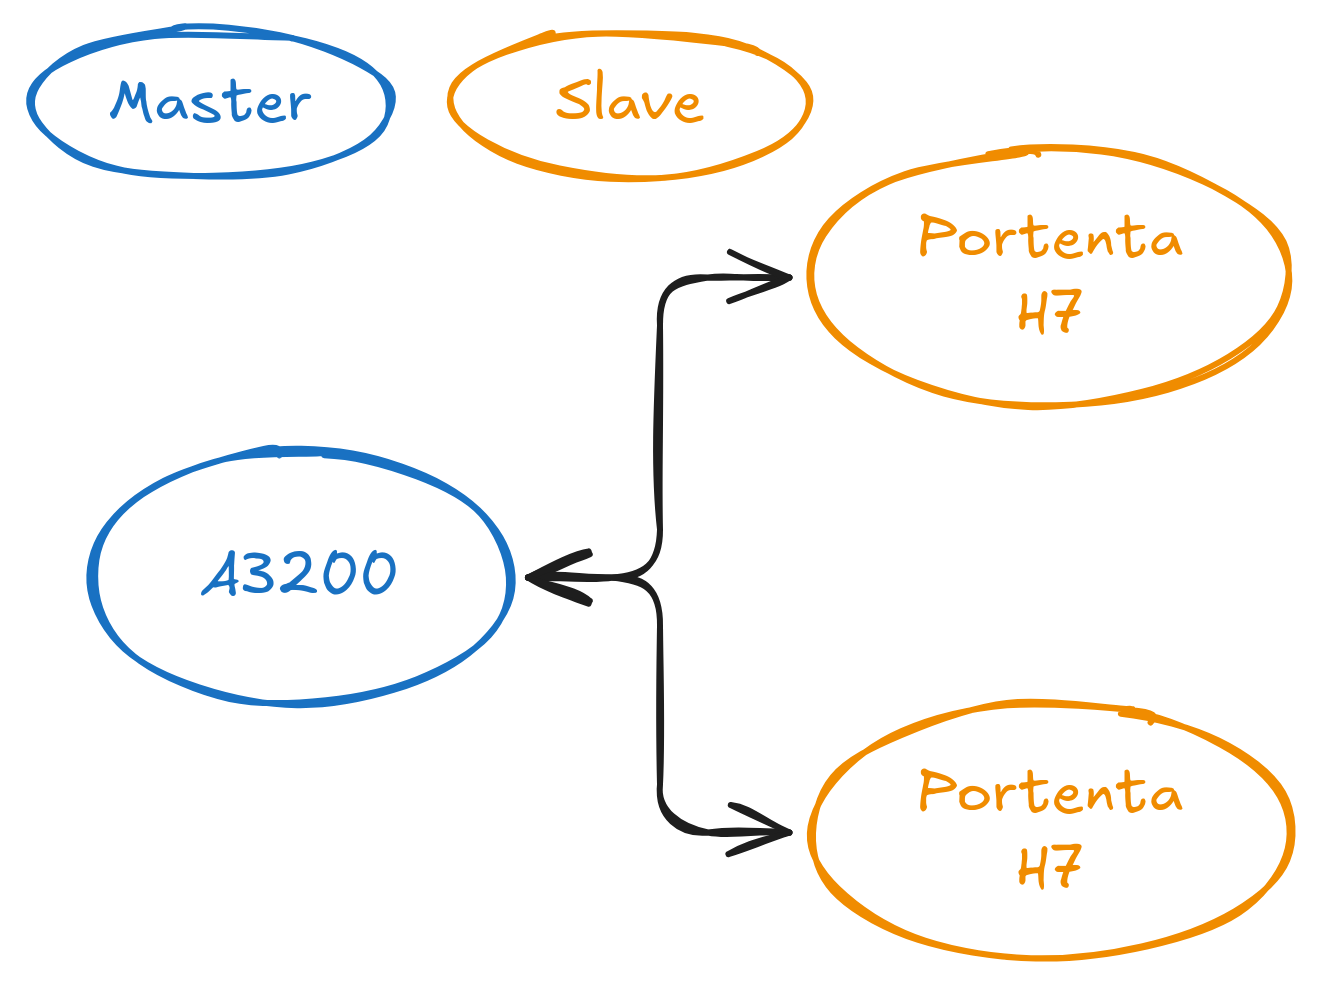
\includegraphics[width=0.6\linewidth]{./images/InternalOBC.png}
  \caption{Comunicación I2C entre computadora primaria y secundaria.}
  \label{fig:i2c_comms}
\end{figure}

Para esta comunicación se utiliza el puerto I2C1 con la siguiente configuración:
\begin{lstlisting}[language=C]
I2C_HandleTypeDef hi2c1;

void MX_I2C1_Init(void) {

  hi2c1.Instance = I2C1;
  hi2c1.Init.Timing = 0x10C0ECFF;
  hi2c1.Init.OwnAddress1 = (0x09 << 1); 
  hi2c1.Init.AddressingMode = I2C_ADDRESSINGMODE_7BIT;
  hi2c1.Init.DualAddressMode = I2C_DUALADDRESS_DISABLE;
  hi2c1.Init.OwnAddress2 = 0;
  hi2c1.Init.OwnAddress2Masks = I2C_OA2_NOMASK;
  hi2c1.Init.GeneralCallMode = I2C_GENERALCALL_DISABLE;
  hi2c1.Init.NoStretchMode = I2C_NOSTRETCH_DISABLE;
  if (HAL_I2C_Init(&hi2c1) != HAL_OK) {
    Error_Handler();
  }
  /** Configure Analogue filter
   */
  if (HAL_I2CEx_ConfigAnalogFilter(&hi2c1, I2C_ANALOGFILTER_ENABLE) != HAL_OK) {
    Error_Handler();
  }
  /** Configure Digital filter
   */
  if (HAL_I2CEx_ConfigDigitalFilter(&hi2c1, 0) != HAL_OK) {
    Error_Handler();
  }
}
\end{lstlisting}

\subsection{UART}

La comunicación UART se utiliza para la comunicación entre la OBC y los demás módulos del satélite, por ejemplo con ADCS, MILO, etc.

% #figure(
%   image("./images/OBCUART.png", width: 60%),
%   caption: [Comunicación UART entre OBC y módulos del satélite.]
% ) <uart_comms>
\begin{figure}[htbp]
  \centering
  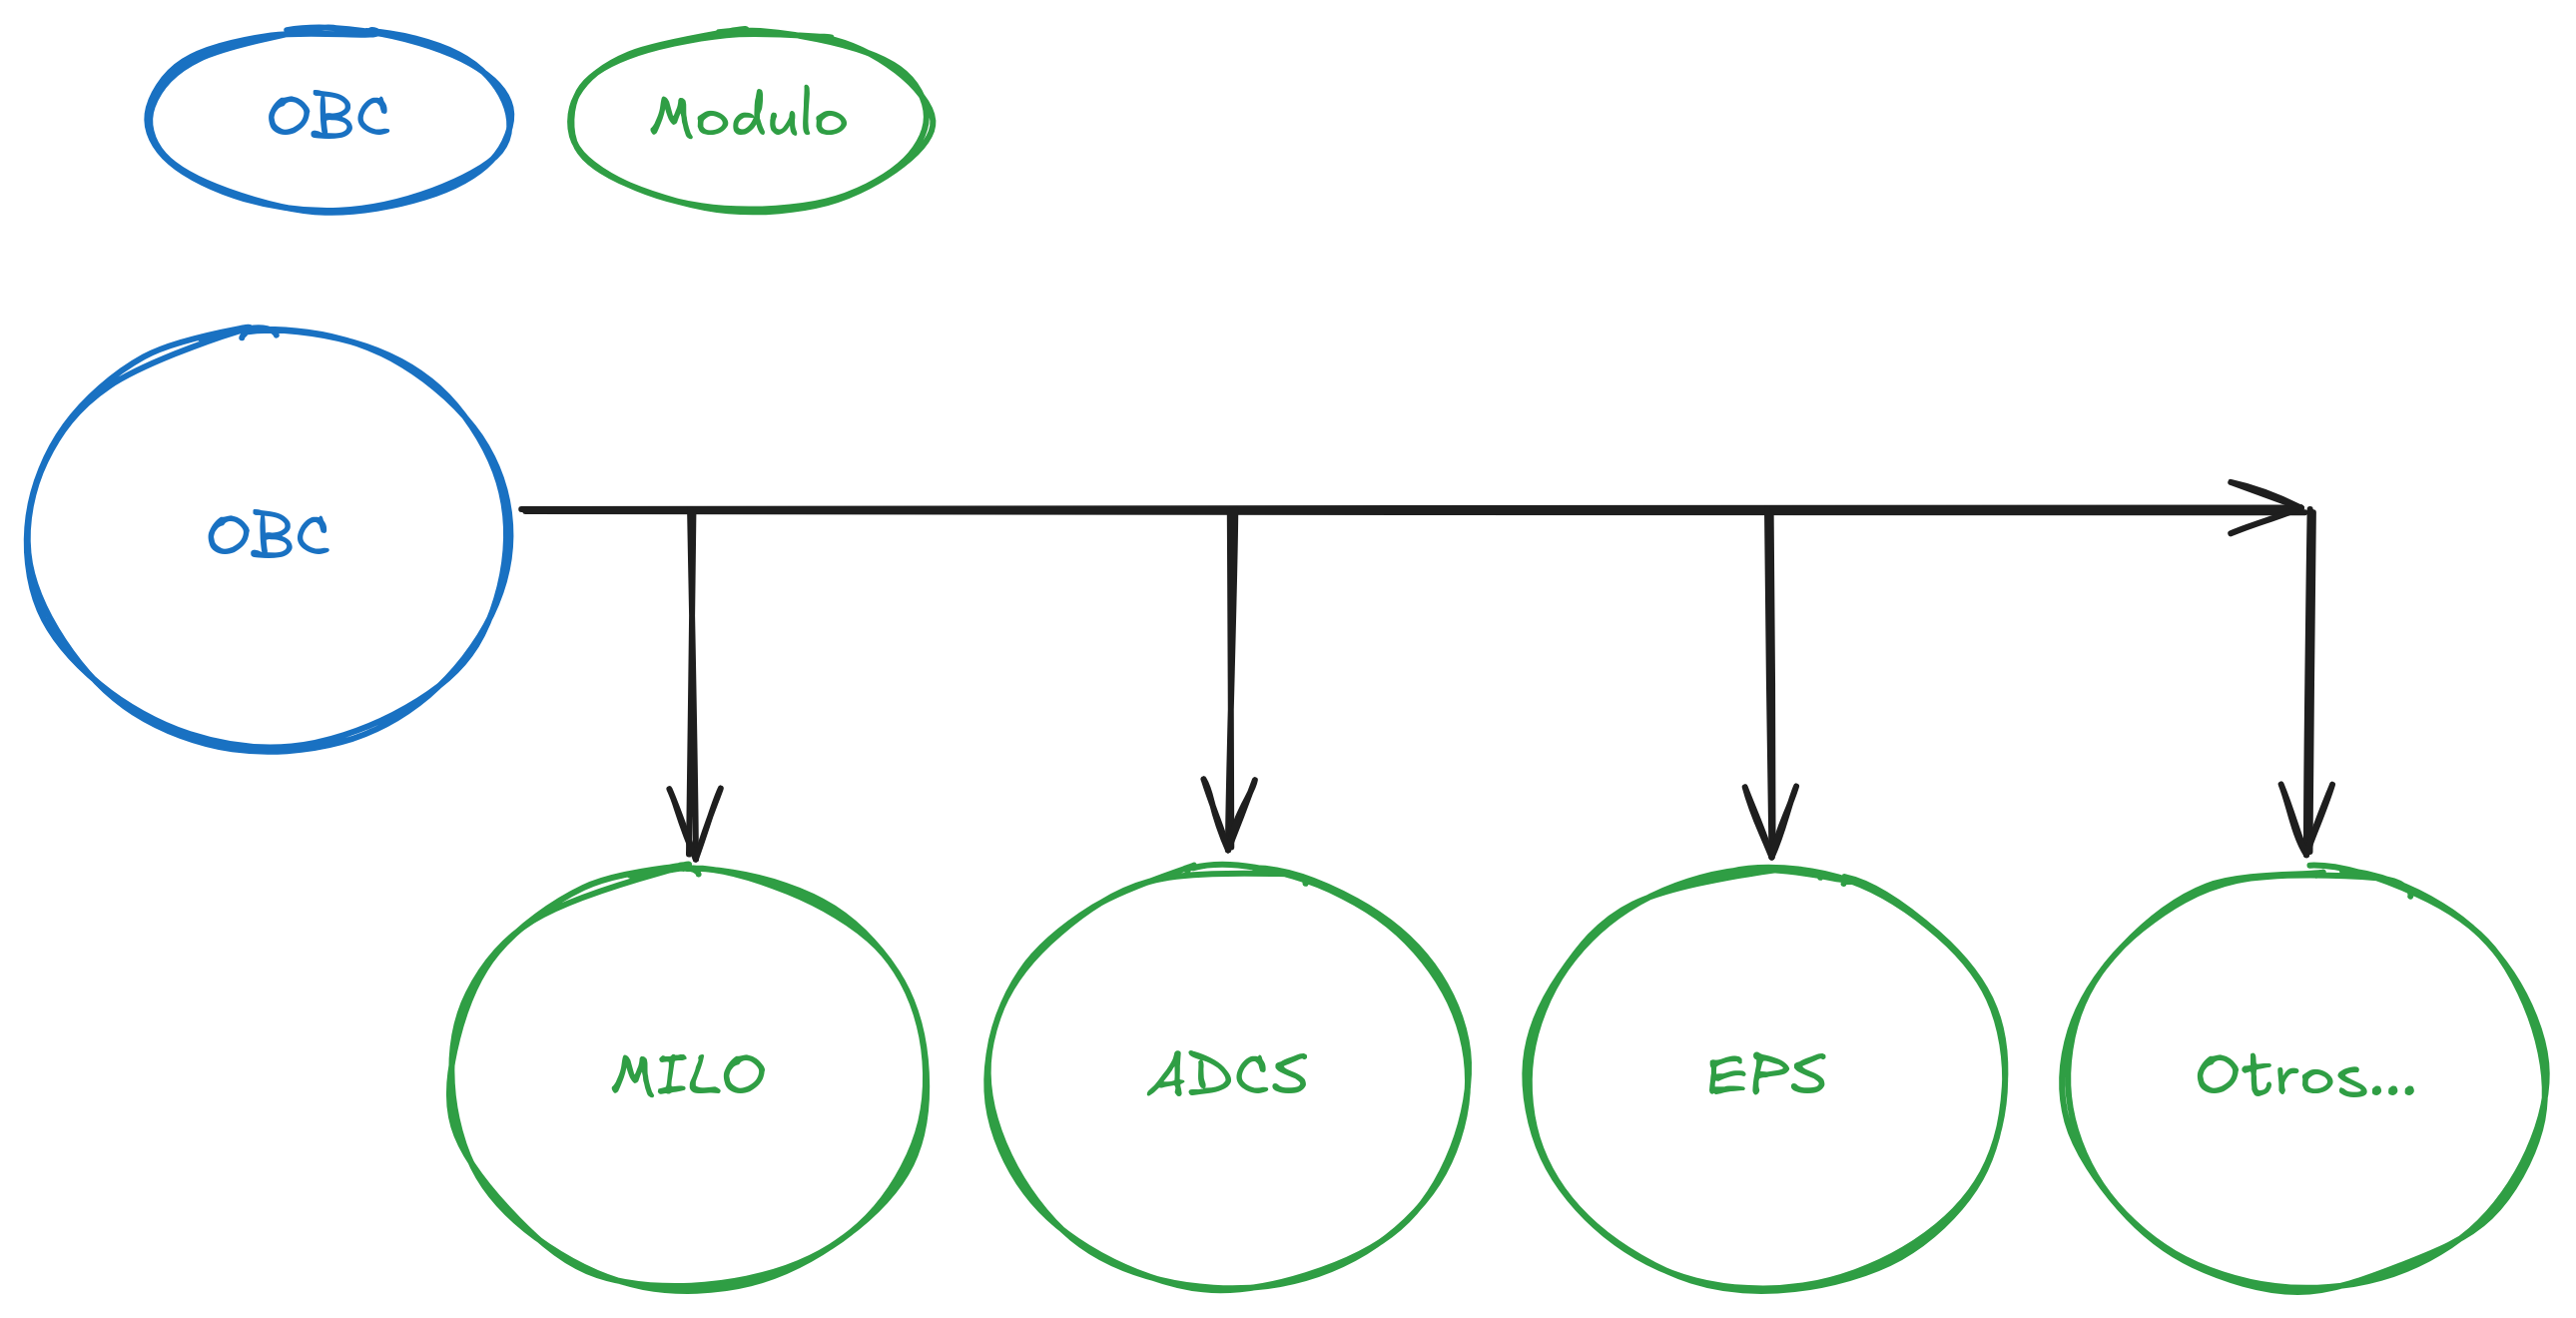
\includegraphics[width=0.6\linewidth]{./images/OBCUART.png}
  \caption{Comunicación UART entre OBC y módulos del satélite.}
  \label{fig:uart_comms}
\end{figure}

Para la comunicación utilizando RS485, se utiliza un puerto en específico de UART: El UART4. Se inicializa de la siguiente manera:
\begin{lstlisting}[language=C]
void MX_UART4_Init(void) {
  huart4.Instance = UART4;
  huart4.Init.BaudRate = 115200;
  huart4.Init.WordLength = UART_WORDLENGTH_8B;
  huart4.Init.StopBits = UART_STOPBITS_1;
  huart4.Init.Parity = UART_PARITY_NONE;
  huart4.Init.Mode = UART_MODE_TX_RX;
  huart4.Init.HwFlowCtl = UART_HWCONTROL_NONE;
  huart4.Init.OverSampling = UART_OVERSAMPLING_16;
  huart4.Init.OneBitSampling = UART_ONE_BIT_SAMPLE_DISABLE;
  huart4.Init.ClockPrescaler = UART_PRESCALER_DIV1;
  huart4.AdvancedInit.AdvFeatureInit = UART_ADVFEATURE_NO_INIT;
  if (HAL_UART_Init(&huart4) != HAL_OK) {
    Error_Handler();
  }
  if (HAL_UARTEx_SetTxFifoThreshold(&huart4, UART_TXFIFO_THRESHOLD_1_8) !=
      HAL_OK) {
    Error_Handler();
  }
  if (HAL_UARTEx_SetRxFifoThreshold(&huart4, UART_RXFIFO_THRESHOLD_1_8) !=
      HAL_OK) {
    Error_Handler();
  }
  if (HAL_UARTEx_DisableFifoMode(&huart4) != HAL_OK) {
    Error_Handler();
  }
}
\end{lstlisting}

La OBC secundaria también utiliza un puerto UART para enviar \textit{logs} con información adicional que aumentan la observabilidad detrás de qué está pasando internamente dentro del sistema, los cuales se pueden leer leyendo el puerto UART6, configurado de la siguiente manera:
\begin{lstlisting}[language=C]
void MX_USART6_UART_Init(void) {
  huart6.Instance = USART6;
  huart6.Init.BaudRate = 115200;
  huart6.Init.WordLength = UART_WORDLENGTH_8B;
  huart6.Init.StopBits = UART_STOPBITS_1;
  huart6.Init.Parity = UART_PARITY_NONE;
  huart6.Init.Mode = UART_MODE_TX_RX;
  huart6.Init.HwFlowCtl = UART_HWCONTROL_NONE;
  huart6.Init.OverSampling = UART_OVERSAMPLING_16;
  huart6.Init.OneBitSampling = UART_ONE_BIT_SAMPLE_DISABLE;
  huart6.Init.ClockPrescaler = UART_PRESCALER_DIV1;
  huart6.AdvancedInit.AdvFeatureInit = UART_ADVFEATURE_NO_INIT;
  if (HAL_UART_Init(&huart6) != HAL_OK) {
    Error_Handler();
  }
  if (HAL_UARTEx_SetTxFifoThreshold(&huart6, UART_TXFIFO_THRESHOLD_1_8) !=
      HAL_OK) {
    Error_Handler();
  }
  if (HAL_UARTEx_SetRxFifoThreshold(&huart6, UART_RXFIFO_THRESHOLD_1_8) !=
      HAL_OK) {
    Error_Handler();
  }
  if (HAL_UARTEx_DisableFifoMode(&huart6) != HAL_OK) {
    Error_Handler();
  }
}
\end{lstlisting}

\section{OBC Secundaria Quetzal-2}

La OBC secundaria se diseñó a nivel de \textit{software} para cumplir los siguientes objetivos, en orden de prioridad:

+ Fiabilidad
+ Seguridad
+ Rendimiento

La OBC secundaria se implementó como una máquina de estados finitos determinista, de esta forma podemos predecir no solo el rendimiento de memoria de la computadora secundaria, sino también su comportamiento. Algunos de los estados de la máquina finita se pueden apreciar en la \ref{fig:finite_state_machine}.

% #mermaid-figure("
% flowchart LR
%     GOM[fa:fa-microchip OBC Principal]-->|Inicia el Handover|Arr
%
%     subgraph fa:fa-microchip OBC Secundaria
%     Arr(fa:fa-diagram-project Arranque de Handover)-->|Inicialización de módulos|Nom(fa:fa-diagram-project Nominal)
%     Nom-->|Comando: Toma de fotografía|MILO(fa:fa-diagram-project Payload MILO)
%     MILO-->|Resultado de la fotografía|Nom
%
%     Nom-->|Comando: Comunicación LORA|LORA(fa:fa-diagram-project Payload LORA)
%     LORA-->|Fin del timeout|Nom
%
%     Nom-->|Comando: ...|OTH(fa:fa-diagram-project Otros subsistemas...)
%     OTH-->|Fin tarea|Nom
%
%     end
%     Nom-->|Fin Handover|GOM
%
%     %% Legend
%   subgraph legend
%     direction LR
%     Y --- |Microchip| Z
%     Z --- |Estado| null
%   end
%   linkStyle 9,10 stroke:#0000,stroke-width:0px;
%
%   classDef hide fill:#0000,stroke:#0000,stroke-width:0px,color:#0000;
%   class legend,null hide;
%   classDef hide-font color:#0000;
%   class Y,Z hide-font;
%
%   class Arr,Nom,MILO,LORA,OTH,Z state
%   class GOM,Y microchip
%
%   classDef microchip fill:lime
%   classDef state fill:yellow
% ",
% caption: [Máquina de Estados Finitos (incompleta) de la OBC secundaria del Quetzal-2. Elaboración propia.],
% alt: "Máquina de Estados Finitos (incompleta) de la OBC secundaria del Quetzal-2. Elaboración propia.",
% ) <finite_state_machine>
\begin{figure}[htbp]
  \centering
  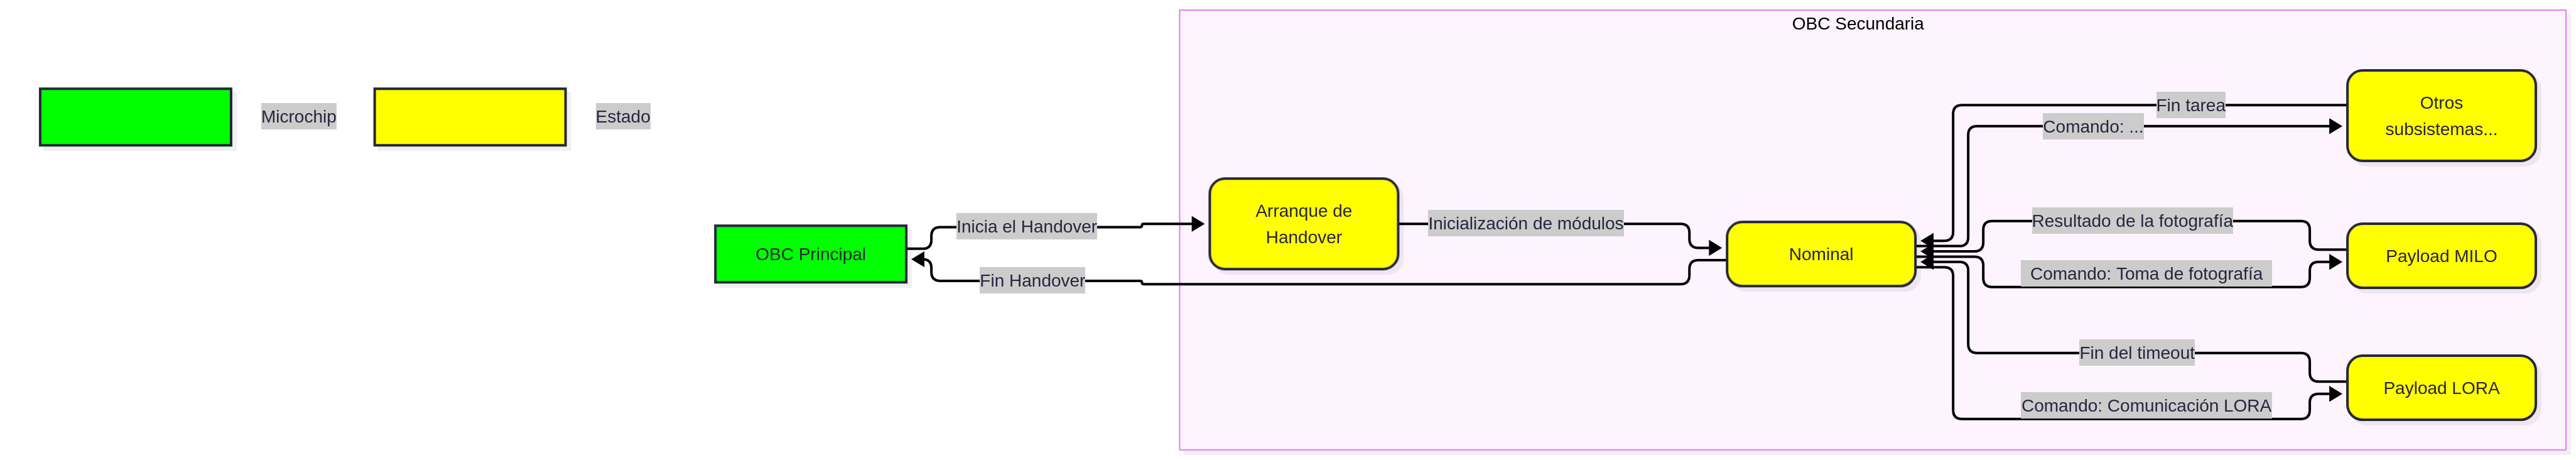
\includegraphics[width=\linewidth]{./images/OBC_FiniteStateMachine.png}
  \caption{Máquina de Estados Finitos (incompleta) de la OBC secundaria del Quetzal-2. Elaboración propia.}
  \label{fig:finite_state_machine}
\end{figure}

Para mejorar el determinismo de esta máquina de estados, todas las tareas que necesitan comunicación con un sistema externo al \textit{core} de la OBC secundaria, por ejemplo interactuar con subsistemas, se realizaron por medio de interfaces. De esta forma se tiene una arquitectura como la descrita en la \ref{fig:hexagonal_arch}.

% #mermaid-figure("
% flowchart LR
%   core(Core OBC)-->rs485(Interfaz RS485)-->milo(Subsistema MILO)
%   rs485-->adcs(Subsistema ADCS)
%   rs485-->adm(Subsistema ADCS)
%
%   core-->i2c(Interfaz I2C)-->gom(OBC Principal)
%
%   core-->uart(Interfaz UART)-->debug(Debug logs)
%
%     %% Legend
%   subgraph legend
%     direction LR
%     Y --- |Interfaz Intermediaria| Z
%     Z --- |Subsistema Interno| null
%   end
%   linkStyle 8,9 stroke:#0000,stroke-width:0px;
%
%   classDef hide fill:#0000,stroke:#0000,stroke-width:0px,color:#0000;
%   class legend,null hide;
%   classDef hide-font color:#0000;
%   class Y,Z hide-font;
%
%   class milo,adcs,adm,gom,debug,Z subsystem
%   class rs485,i2c,uart,Y interface
%
%   classDef interface fill:lime
%   classDef subsystem fill:yellow
% ",
% caption: [Arquitectura de la OBC secundaria. Elaboración propia.],
% alt: "Arquitectura de la OBC secundaria. Elaboración propia.",
% ) <hexagonal_arch>
\begin{figure}[htbp]
  \centering
  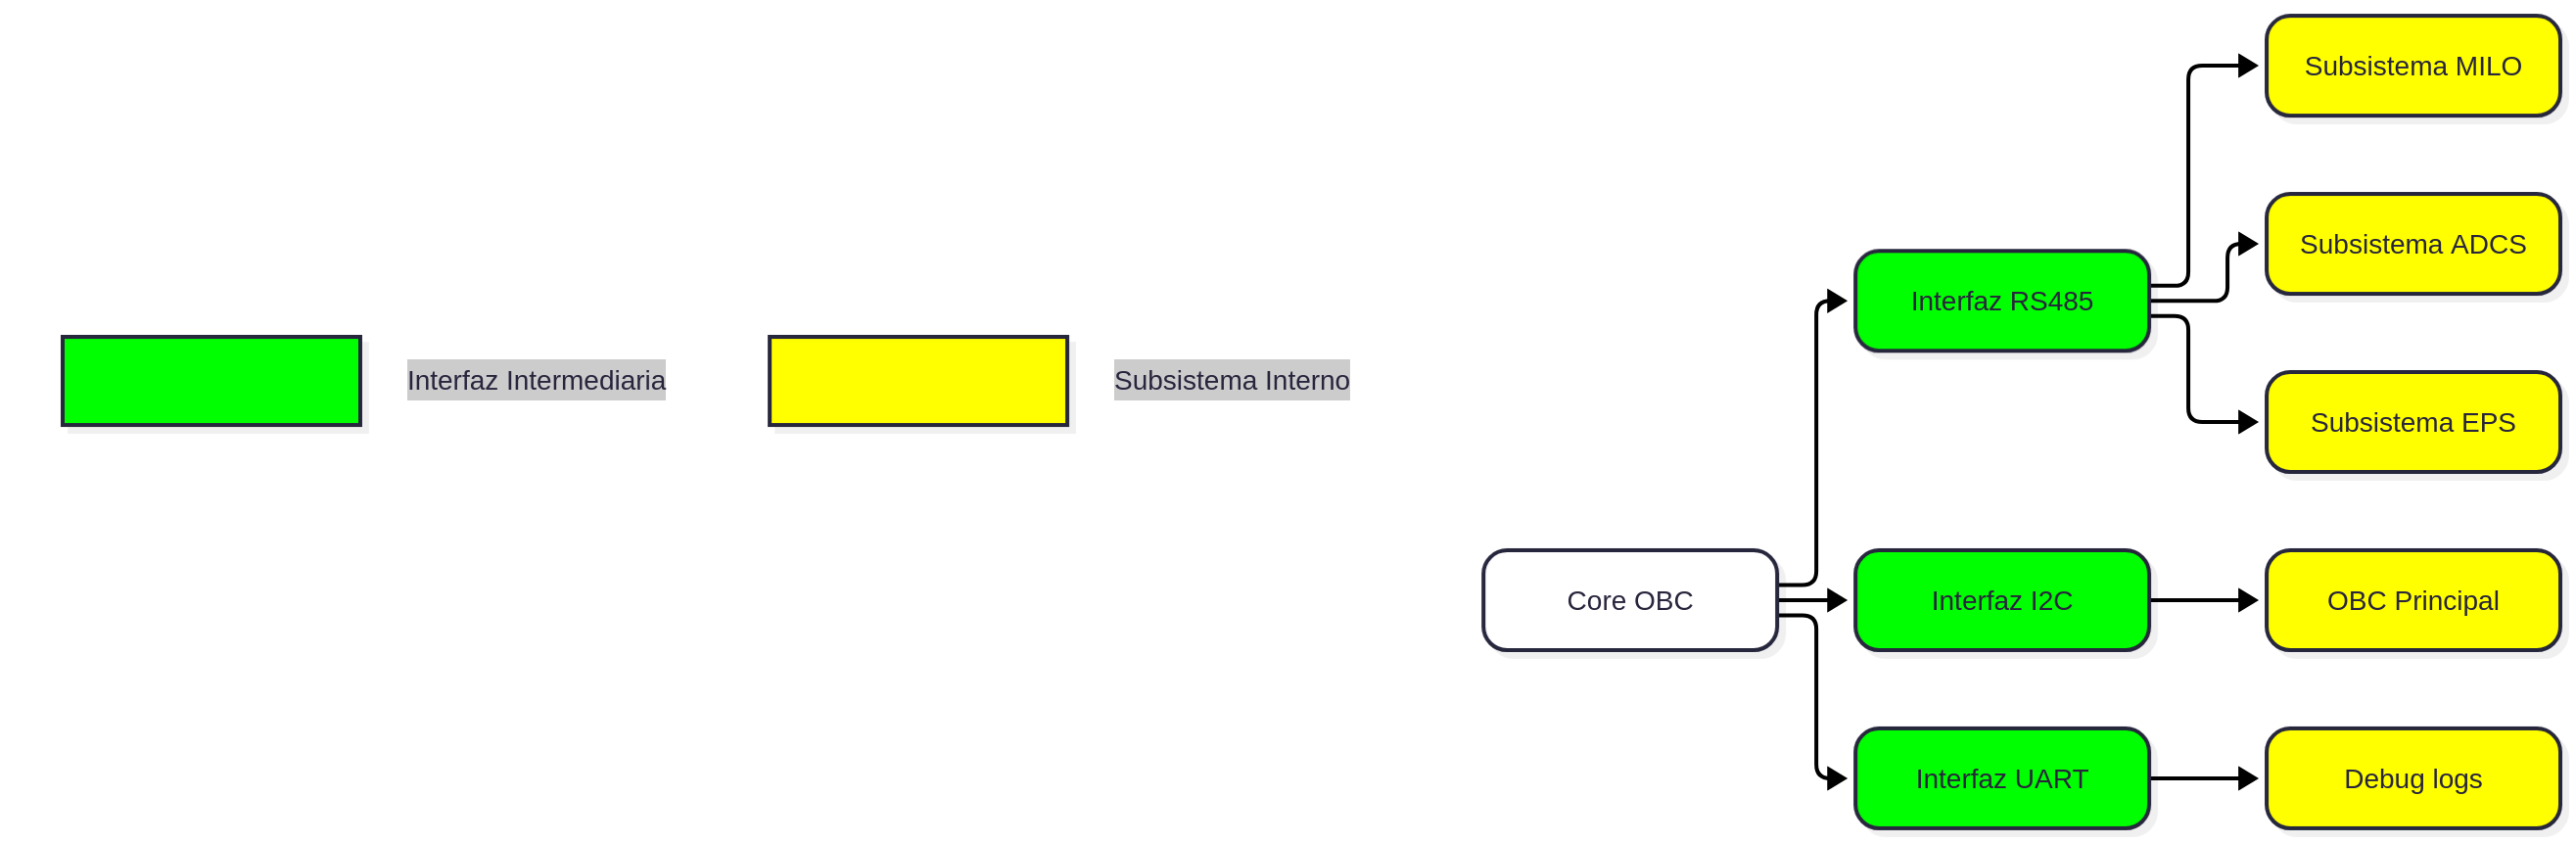
\includegraphics[width=\linewidth]{./images/Hexagonal_arch.png}
  \caption{Arquitectura de la OBC secundaria. Elaboración propia.}
  \label{fig:hexagonal_arch}
\end{figure}

Esta arquitectura de la \ref{fig:hexagonal_arch} nos permitió varias bondades:
- Nos permitió intercambiar todos los subsistemas (en amarillo) por implementaciones que funcionen o fallen de formas predecibles.
- Se logró simular entradas y salidas de los distintos subsistemas a voluntad sin necesidad de conectar físicamente todo el sistema o que siquiera se encuentre desarrollado.
- Se automatizaron las pruebas de comportamiento de la OBC ante una gran variedad de entradas de los distintos submódulos.
- Automatización de generación de casos de prueba con \textit{fuzzing} en AFL++.

\chapter{Resultados}
% #figure(
%   image("./images/HandoverTest.jpeg"),
%   caption: [Prueba del protocolo de handover corriendo localmente dentro de una misma computadora.]
% ) <laptop_test>
\begin{figure}[htbp]
  \centering
  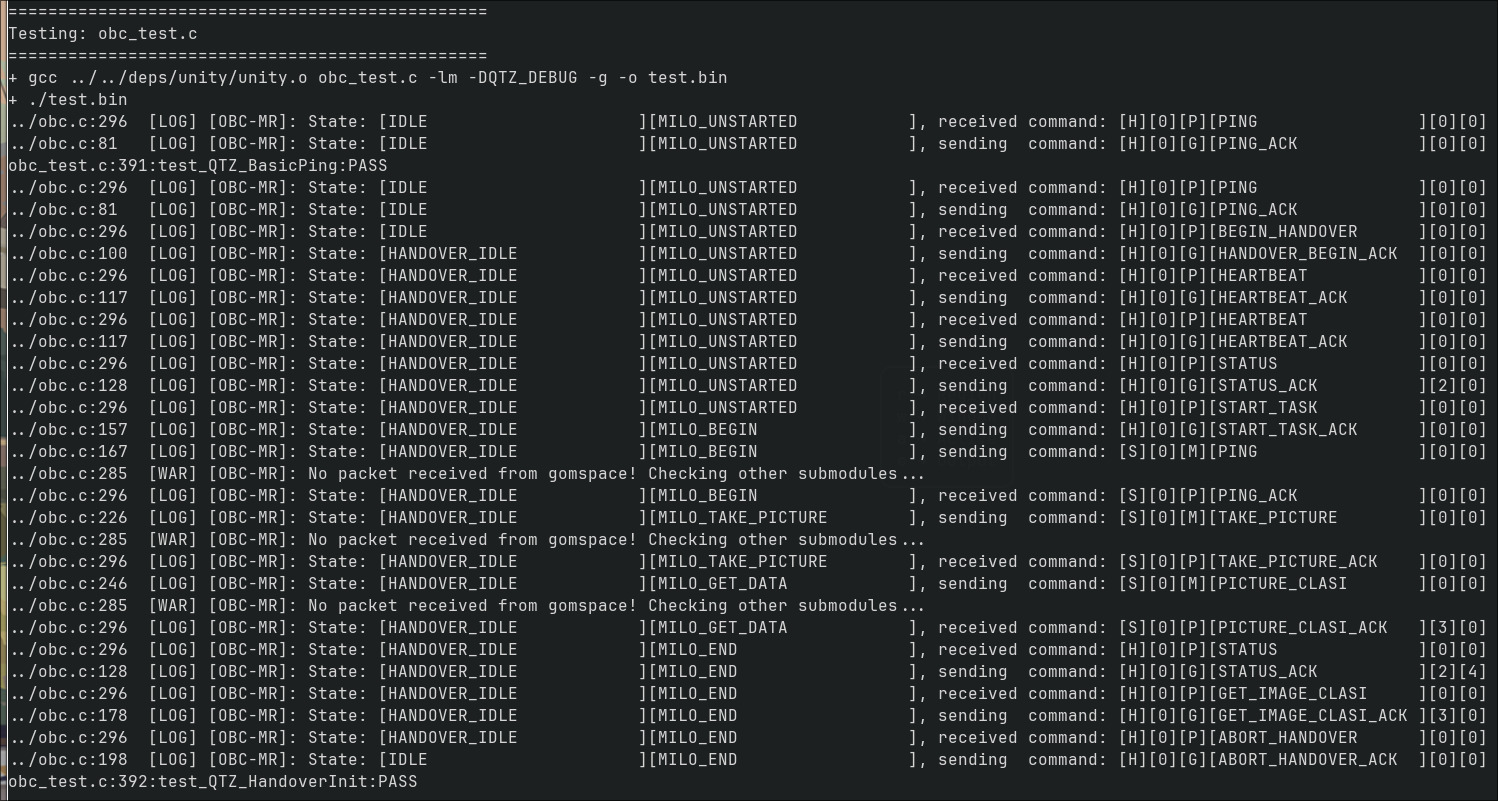
\includegraphics[width=\linewidth]{./images/HandoverTest.jpeg}
  \caption{Prueba del protocolo de handover corriendo localmente dentro de una misma computadora.}
  \label{fig:laptop_test}
\end{figure}

%
% #figure(
%   image("./images/HandoverLowQuality.jpeg", width: 60%),
%   caption: [Prueba del protocolo de handover corriendo con hardware real entre la computadora primaria y secundaria. _Logs_ desde la perspectiva de la OBC secundaria.]
% ) <handover_test>
\begin{figure}[htbp]
  \centering
  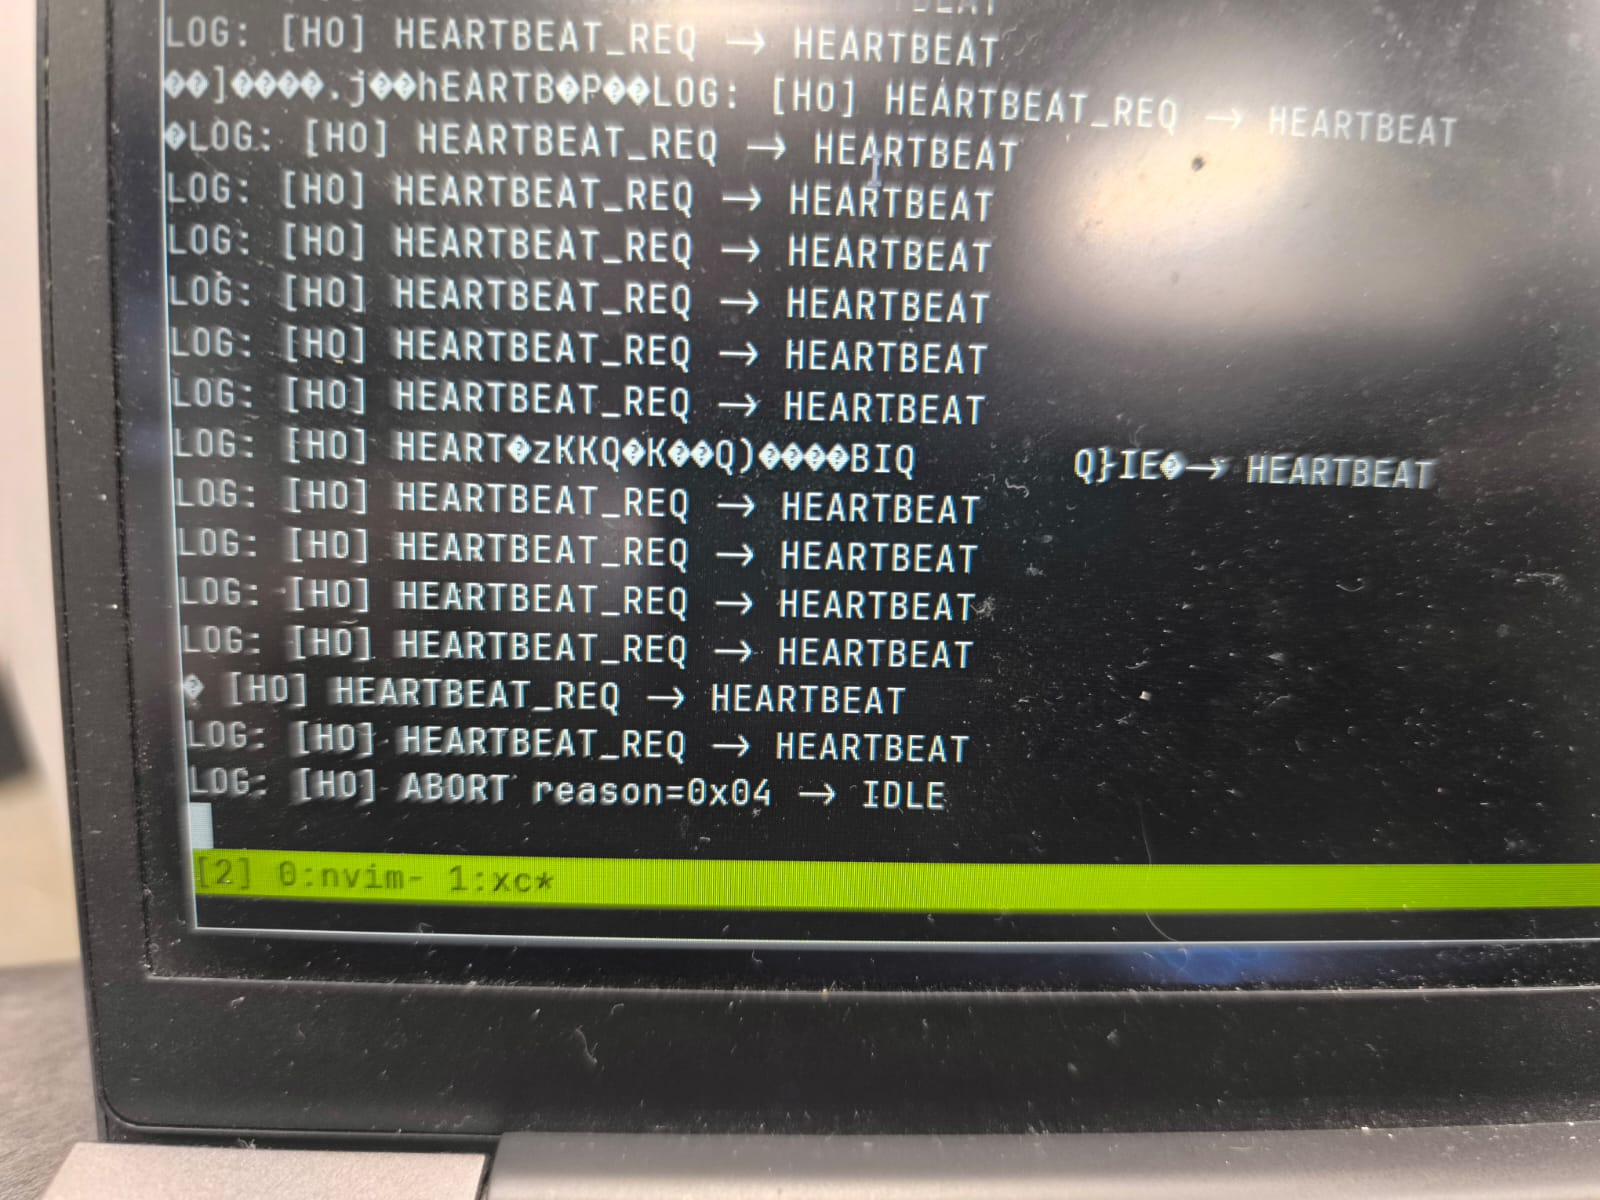
\includegraphics[width=0.6\linewidth]{./images/HandoverLowQuality.jpeg}
  \caption{Prueba del protocolo de handover corriendo con hardware real entre la computadora primaria y secundaria. \textit{Logs} desde la perspectiva de la OBC secundaria.}
  \label{fig:handover_test}
\end{figure}

%
% #figure(
%   image("./images/Command_reception.jpeg", width: 60%),
%   caption: [Prueba del protocolo de handover corriendo con hardware real entre la computadora primaria y secundaria. Realizado durante la visita de David Cuartielles, cofundador de Arduino y Andrés Sabas, fundador de Electronic Cats.]
% ) <command_reception>
\begin{figure}[htbp]
  \centering
  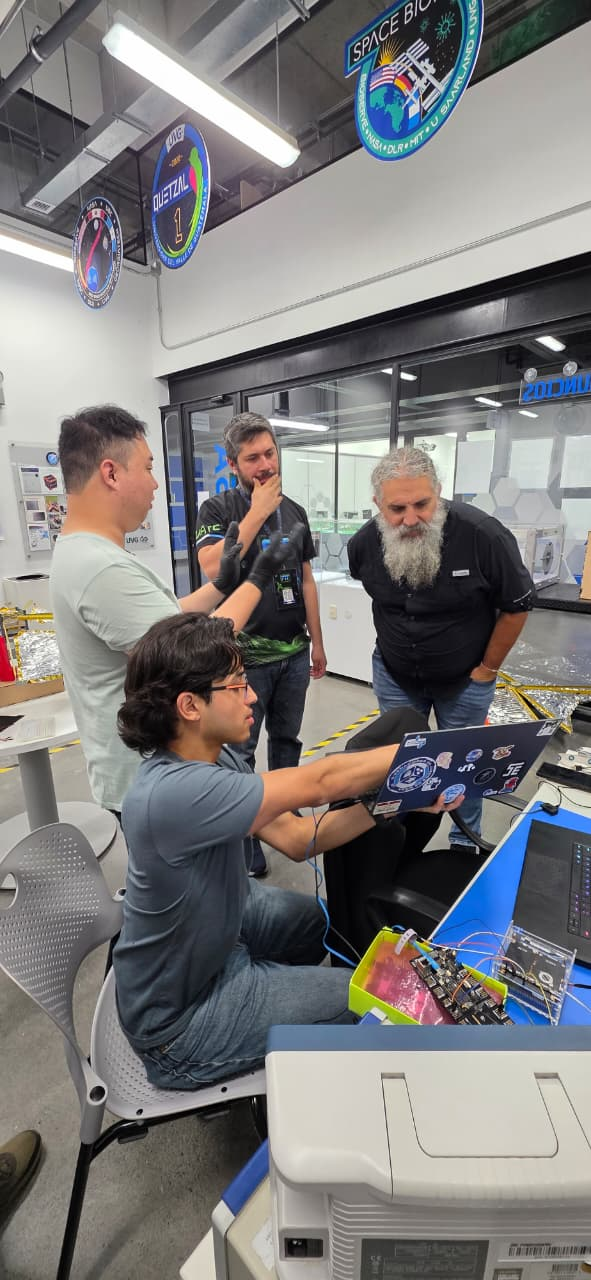
\includegraphics[width=0.6\linewidth]{./images/Command_reception.jpeg}
  \caption{Prueba del protocolo de handover corriendo con hardware real entre la computadora primaria y secundaria.}
  \label{fig:command_reception}
\end{figure}

%
% #figure(
%   image("./images/milo.jpeg", width: 60%),
%   caption: [Fotografía tomada con la _Payload MILO_ durante la prueba de handover.]
% ) <milo_picture>
\begin{figure}[htbp]
  \centering
  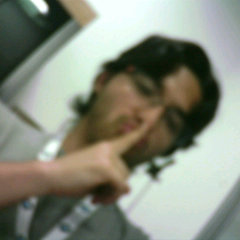
\includegraphics[width=0.6\linewidth]{./images/milo.jpeg}
  \caption{Fotografía tomada con la \textit{Payload MILO} durante la prueba de handover.}
  \label{fig:milo_picture}
\end{figure}

\begin{figure}[htbp]
  \centering
  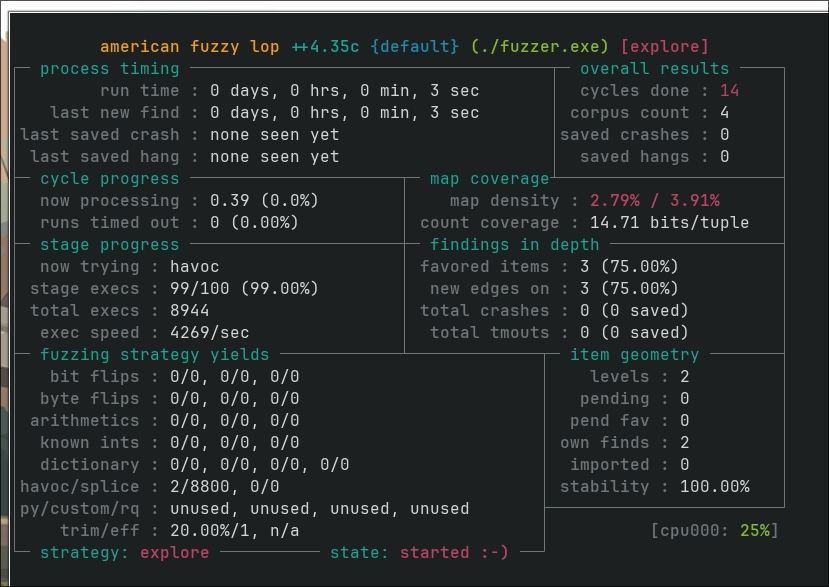
\includegraphics[width=\linewidth]{./images/OBC_Fuzzing.jpg}
  \caption{\textit{Fuzzing} del core de la OBC.}
  \label{fig:obc_fuzzing}
\end{figure}

\begin{figure}[htbp]
  \centering
  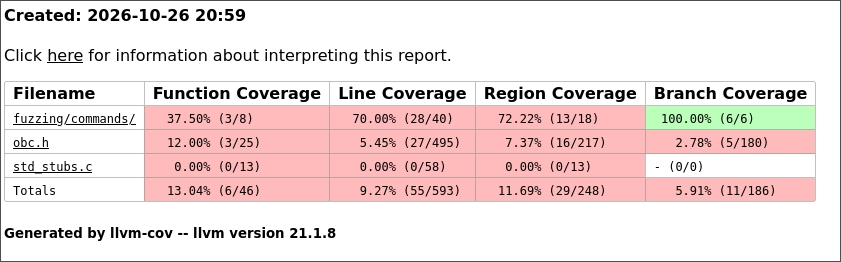
\includegraphics[width=\linewidth]{./images/OBC_Coverage.jpg}
  \caption{\textit{Coverage Report} del fuzzing del core de la OBC.}
  \label{fig:obc_coverage}
\end{figure}

\newpage
\chapter{Discusión de Resultados}
Como se puede apreciar en la \ref{fig:laptop_test}, se realiza el camino sin errores de una rutina de handover completa, desde que la OBC primaria solicita el traslado de poder, pasando por el inicio de la tarea de MILO en donde se toma la fotografía y finalizando con el comando de abortar de la OBC primaria.

Toda esa rutina se ejecutó dentro de un ambiente simulado en la computadora, y cada una de las respuestas y acciones que decidía tomar la OBC secundaria fue analizada por la prueba, solamente retornando éxito si todos los comandos recibidos y enviados seguían la especificación del protocolo interno. Es decir, la prueba revisó que luego de recibir el comando \texttt{BEGIN\_HANDOVER} desde la computadora principal, la OBC secundaria respondiera con \texttt{BEGIN\_HANDOVER\_ACK}. No solo se limitó a revisar el estado, sino que además revisa cada uno de los \textit{bytes} de la respuesta y el largo configurado por el \textit{buffer} de salida.

Nótese el cambio de estados dentro de la OBC secundaria que se puede apreciar en los \textit{logs}, iniciando en \texttt{IDLE} para transicionar a \texttt{HANDOVER\_IDLE} y finalmente a \texttt{IDLE} de nuevo. Estos son los estados principales de la OBC secundaria, mientras que el estado interno de la tarea es \texttt{MILO\_UNSTARTED}. La combinación de estos dos estados (\texttt{IDLE}, \texttt{MILO\_UNSTARTED}) representan el modo de operación de arranque dentro del Producto Mínimo Viable (MVP por sus siglas en inglés) de la OBC secundaria. Para luego transicionar al estado nominal (\texttt{HANDOVER\_IDLE}, \texttt{MILO\_UNSTARTED}), para finalmente llegar al estado de toma de fotografía (\texttt{HANDOVER\_IDLE}, \texttt{MILO\_BEGIN}). La \ref{fig:obc_states} muestra en forma de diagrama estas transiciones:

% #figure(
%   image("./images/OBC_States.png", width: 80%),
%   caption: [Estados de la OBC secundaria de estados finitos.]
% ) <obc_states>
\begin{figure}[htbp]
  \centering
  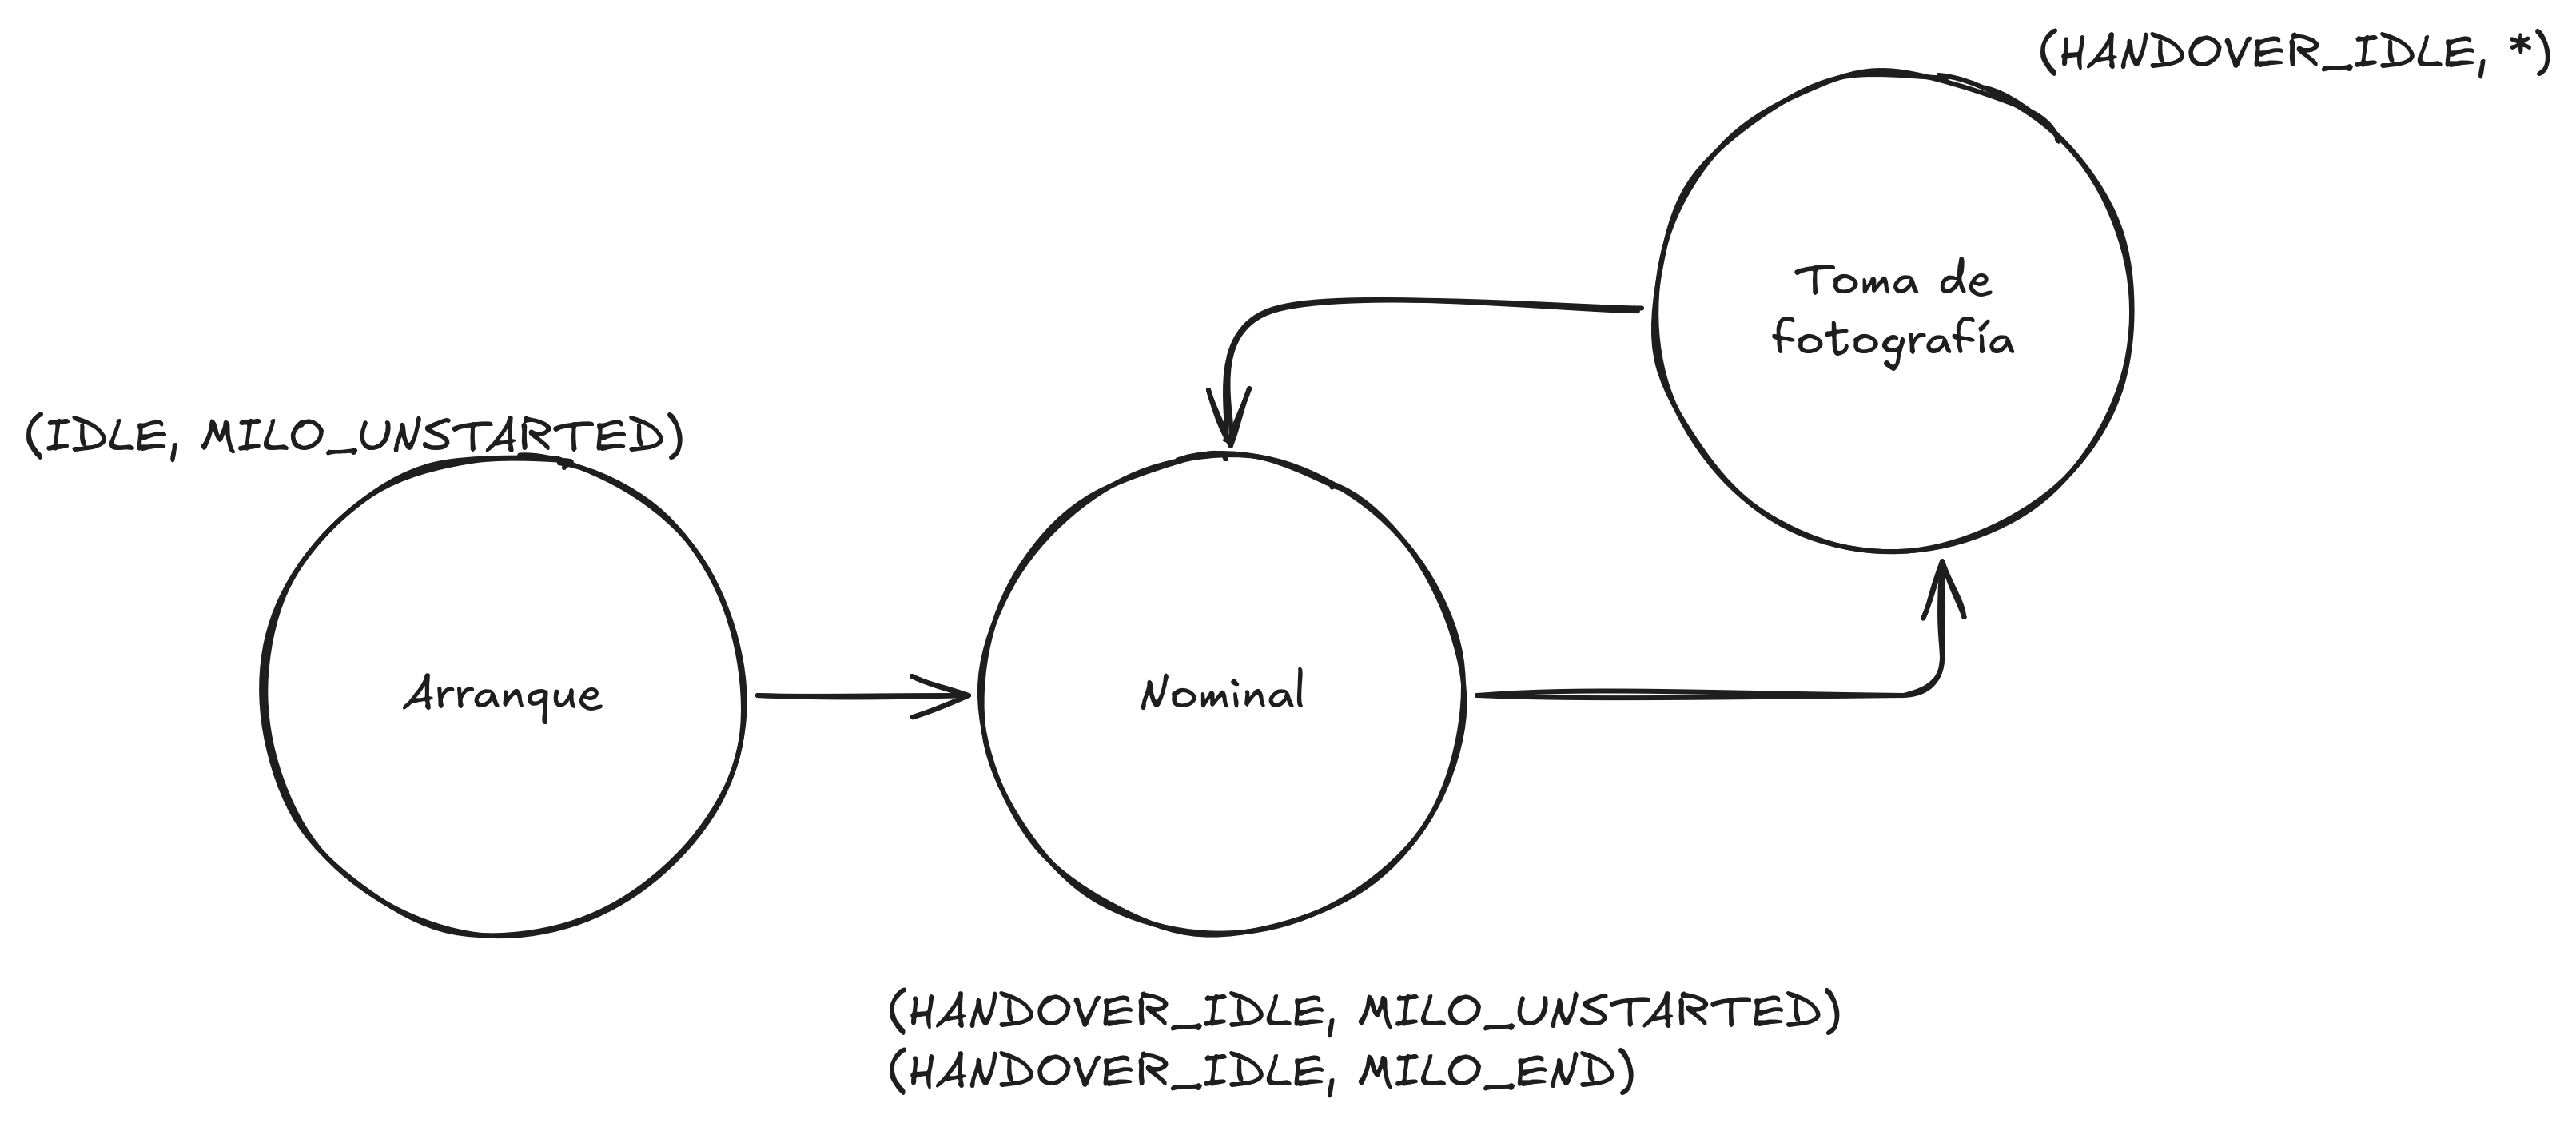
\includegraphics[width=0.8\linewidth]{./images/OBC_States.png}
  \caption{Estados de la OBC secundaria de estados finitos.}
  \label{fig:obc_states}
\end{figure}

Esta es la prueba principal que se implementó, pero gracias a la arquitectura hexagonal se tiene la posibilidad de implementar muchas más que prueben casos más extraños, o simplemente probar casos de error que permitan asegurar que la OBC fallará de una manera predecible cuando se cumplan ciertas condiciones. Esto es parte de las opciones de \textit{testing} que se vieron en el capítulo \ref{sec:reliability}.

Además, se utilizó AFL++ para implementar un \textit{fuzzer} básico de la rutina principal de la OBC secundaria (\ref{fig:obc_fuzzing}), en la imagen en cuestión se puede apreciar que el \textit{fuzzer} lleva corriendo apenas 3 segundos pero ya corrió más de 8900 veces la rutina principal. De las cuales ha encontrado 3 nuevas aristas pero no ha encontrado \textit{crashes} todavía. El \textit{harness} programado para esta sesión de \textit{fuzzing} es limitado, de hecho podemos ver en \ref{fig:obc_coverage} que este \textit{harness} no es particularmente bueno, puesto que solamente 5 de 180 ramas que componen la rutina principal fueron invocadas durante esta sesión. Lo cual es esperado debido a que el \textit{harness} configurado para esta prueba es una prueba de concepto, su función principal es validar que la arquitectura efectivamente se puede utilizar para pruebas avanzadas de código que verifiquen su fiabilidad.

El que la prueba mostrada en la \ref{fig:laptop_test} tenga un resultado satisfactorio no significa que la OBC secundaria funcione, puesto que es un ambiente simulado dentro de la misma computadora. Por esto se realizaron pruebas con implementaciones reales de las interfaces, las cuales se pueden ver en la \ref{fig:handover_test} y la \ref{fig:command_reception}. En esta prueba se intentó solamente la comunicación entre los dos módulos de la OBC, primaria y secundaria. Como se puede ver en los \textit{logs}, la comunicación fue satisfactoria y se logró llegar al último comando de aborto del protocolo de handover.

Finalmente, en la \ref{fig:milo_picture} se puede apreciar la fotografía de una prueba final con todos los subsistemas conectados utilizando las implementaciones reales de las interfaces de comunicación. La imagen se encuentra borrosa debido a la configuración de la cámara, ya que se tenía en baja calidad para limitar la cantidad de espacio que cada fotografía consumía al ser almacenada y transmitida dentro del sistema. Para ese punto de las pruebas lo importante no era la calidad de las fotografías sino que el sistema pudiera tomarla de forma autónoma.
